\documentclass[border=6pt]{standalone}
\usepackage{amsmath}
\usepackage{amssymb}
\usepackage{tikz}
\usepackage{pgfplots}
\pgfplotsset{compat=1.18}
\usetikzlibrary{arrows.meta,calc,positioning}
\begin{document}
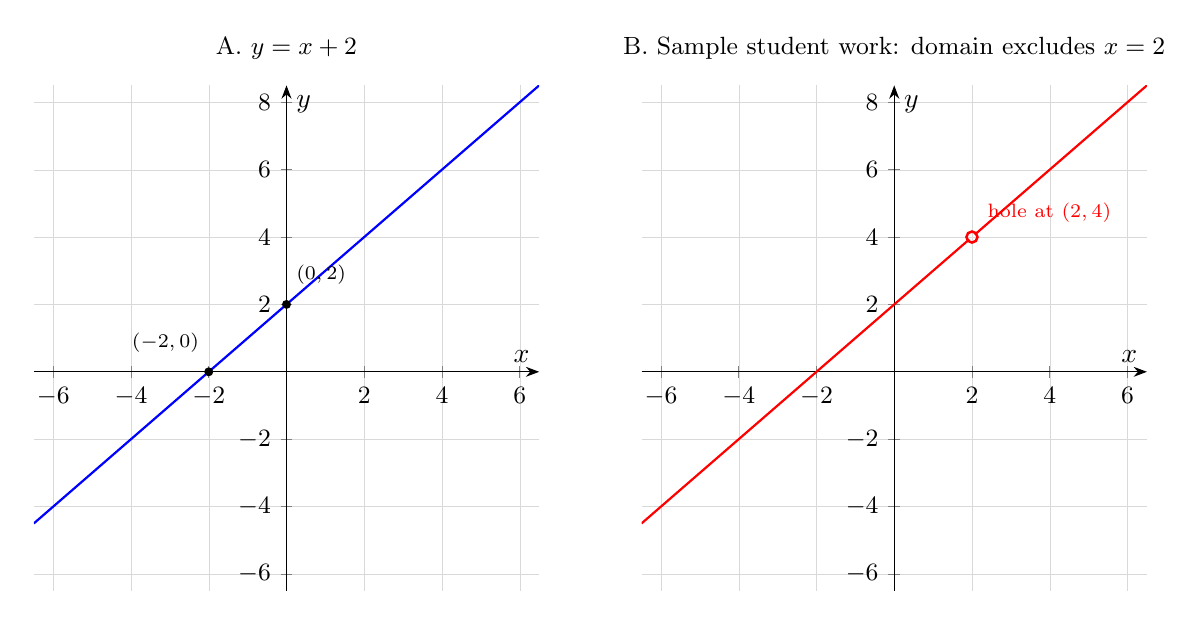
\begin{tikzpicture}
\begin{axis}[name=ax1,
    axis lines = middle,
    xlabel = {$x$}, ylabel = {$y$},
    grid=both,
    grid style={line width=.1pt, draw=gray!30},
    axis line style={-Stealth},
    legend style={font=\small},
    tick label style={font=\small},
    xmin=-6.5, xmax=6.5, ymin=-6.5, ymax=8.5,
    xtick={-6,-4,-2,0,2,4,6},
    ytick={-6,-4,-2,0,2,4,6,8},
    width=8cm, height=8cm,
    title={\small A. $y=x+2$},
]
\addplot[domain=-6.5:6.5, samples=2, thick, blue] {x+2};
\addplot[only marks, mark=*, mark size=1.4pt, black] coordinates {(-2,0) (0,2)};
\node[anchor=south east, font=\scriptsize] at (axis cs:-2,0.3) {$(-2,0)$};
\node[anchor=south west, font=\scriptsize] at (axis cs:0,2.3) {$(0,2)$};
\end{axis}
\begin{axis}[at={(ax1.south east)}, anchor=south west, xshift=1.3cm,
    axis lines = middle,
    xlabel = {$x$}, ylabel = {$y$},
    grid=both,
    grid style={line width=.1pt, draw=gray!30},
    axis line style={-Stealth},
    legend style={font=\small},
    tick label style={font=\small},
    xmin=-6.5, xmax=6.5, ymin=-6.5, ymax=8.5,
    xtick={-6,-4,-2,0,2,4,6},
    ytick={-6,-4,-2,0,2,4,6,8},
    width=8cm, height=8cm,
    title={\small B. Sample student work: domain excludes $x=2$},
]
\addplot[domain=-6.5:1.93, samples=2, thick, red] {x+2};
\addplot[domain=2.07:6.5, samples=2, thick, red] {x+2};
\addplot[only marks, mark=o, mark size=2pt, mark options={fill=white, draw=red, line width=0.9pt}] coordinates {(2,4)};
\node[anchor=south west, font=\scriptsize, red] at (axis cs:2.15,4.15) {hole at $(2,4)$};
\end{axis}
\end{tikzpicture}
\end{document}
